\scanpage{73}
(soit $U=f(\mathbb D^\circ)$)

\figure{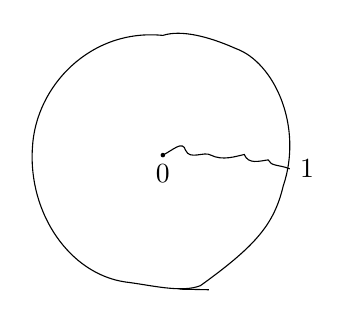
\begin{tikzpicture}[scale=.76]
\draw (0,2) .. controls (-1.20,2.12) and (-2.13,1.16) .. (-2.18,.12) .. controls (-2.25,-.96) and (-1.57,-1.98) .. (-.63,-2.12) .. controls (-.21,-2.17) and (.32,-2.31) .. (.63,-2.18) .. controls (1.56,-1.51) and (1.86,-1.15) .. (2.01,-.52) .. controls (2.35,.48) and (1.86,1.55) .. (1.22,1.78) .. controls (.77,1.98) and (.31,2.10) .. (0,2);
\draw (0,0) .. controls (.18,.09) and (.33,.25) .. (.38,.08) .. controls (.45,-.09) and (.69,.07) .. (.80,0) .. controls (1,-.10) and (1.22,-.02) .. (1.36,.01) .. controls (1.43,-.16) and (1.61,-.10) .. (1.76,-.08) .. controls (1.80,-.19) and (1.96,-.16) .. (2.12,-.23);
\fill (0,0) circle (.038) node[below]{$0$};\node[right] at (2.13,-.23){$1$};
\draw (.28,-2.24)--(.77,-2.25);
\end{tikzpicture}}

2) $f(0)=0$, $f(\zeta)=f(\bar\zeta)=1$
\deleted{3) $f\mid\unsure{\beta|\alpha}$ est un}
$f\mid(\alpha\setminus\{\zeta,\bar\zeta))$ \deleted{est} \inserted{induit} un
homéo avec $\partial\mathbb D\setminus\{1\}$

3) $\deleted{f\mid[1,\zeta\mathclose{\unsure{[|]}}}$ $f\mid\beta$ et $f\mid\bar\beta$ sont injectives et
ont $=$ image, \deleted{qui \unsure{est|contient}, et $I\setminus\{1\}$} \inserted{$I$, contenant $\{1\}$} d'après
2) et $I\setminus\{1\}$ est contenu dans $\mathbb D^\circ$.

4) Soient $f_1:\beta\xrightarrow{\sim}I$, $f_2:\bar\beta\xrightarrow{\sim}I$ induits par $f$,
\inserted{alors $\varphi=f_2^{-1}f_1$}

\uline{NB} Ici encore, $f$ est unique. On peut
résumer ce théorème d'uniformisation
avec bord dans le \deleted{Scholie}

\uline{Scholie} Il y a corr. 1-1 entre les
données suivantes :

a) Les homéos rectifiables \deleted{\unsure{croi}}
\[
\begin{aligned}
\psi:[0,1]\simeq[0,1] &\qquad\text{avec }\psi(0)=0\\
&\qquad\text{donc }\psi(1)=1
\end{aligned}
\]

b) Les segments topologiques \uline{rectifiables}
$I$ dans $\mathbb D$, tels que \deleted{$I\cap\partial\mathbb D$ soit réduit
à une extrémité de $I$} \inserted{$I$ admette $0,1$ comme}
extrémités et \deleted{$I\setminus\{1\}\unsure{\subset|=}\unsure{1}$}
$I\cap\partial\mathbb D=\{1\}$ (i.e.
$I\setminus\{1\}\subset\mathbb D^\circ\}$

c) Les \deleted{\unsure{ap}} applications continues $f:\mathbb D\mathrel{\unsure{-|\to}}\mathbb D$
qui ont les propriétés 1) 2) 3) de B) ci-dessus
% archive sheet number: 75
